\documentclass[xcolor=svgnames, t]{beamer}

\usepackage[utf8]{inputenc}
% \usepackage{booktabs, comment}
\usepackage[absolute, overlay]{textpos}
\useoutertheme{infolines} 
% \usepackage{csquotes}
\usepackage{enumerate}
\usepackage[french]{babel}
\usepackage{xcolor}
% \usepackage[citestyle=authoryear,backend=bibtex,citetracker=true]{biblatex}
% \bibliography{bibfile}

% \usepackage{mathabx}
% \newcommand{\stup}{{\scriptsize $\blacktriangle$ }}
% \newcommand{\stdown}{$\blacktriangledown$ }
\newcommand{\eg}{\textit{e.g. }}
\newcommand{\ie}{\textit{i.e. }}
\renewcommand{\footnotesize}{\tiny}
\newcommand{\coloredemph}[1]{\textcolor{internationalblue}{\emph{#1}}}
% \newcommand{\Rlogo}{\includegraphics[scale = 0.02]{images/Rlogo.png}}
% \newcommand{\Pythonlogo}{\includegraphics[scale = 0.075]{images/Pythonlogo.png}}

% math commands
\usepackage{amsmath}
\newcommand{\norm}[2]{\lVert #1 \rVert_{#2}}
\newcommand{\dictx}{\mathbf{\Theta}_{X_n}}
\newcommand{\vectorx}[1]{\boldsymbol{\MakeLowercase{\mathbf{#1}}}}
\newcommand{\matrixx}[1]{\boldsymbol{\MakeUppercase{#1}}}
\newcommand{\argmin}{\mathop{\mathrm{arg\,min}}}
\newcommand{\argmax}{\mathop{\mathrm{arg\,max}}}
\newcommand{\argminx}[1]{\arg\min_{#1}}
\newcommand{\dotprod}[2]{\langle #1, #2 \rangle}
\newcommand{\scalemath}[2]{\scalebox{#1}{\mbox{\ensuremath{\displaystyle #2}}}}

% Images location
\graphicspath{ {./images/} }

\definecolor{myuniversity}{RGB}{36, 42, 117}
\definecolor{internationalblue}{RGB}{48, 157, 181}
\definecolor{dodgerblue}{RGB}{91, 193, 213}
\usecolortheme[named=myuniversity]{structure}
\usepackage{tikz}

\usetheme{Madrid}

\logo{\includegraphics[scale=0.25]{Thales.png}}
\setbeamercolor{title in head/foot}{bg=internationalblue}
\setbeamercolor{author in head/foot}{bg=dodgerblue}

\title[Introduction aux Processus Gaussiens]{Introduction aux Processus Gaussiens}
\subtitle{Application aux données spatio-temporelles}
\institute[]{}
% \titlegraphic{
% 	\includegraphics[scale=0.5]{Thales.png}
% % 	\includegraphics[height=1.5cm]{images/UT3_PRES_logoQ.png}
% }
\author[Cl\'ement Lejeune]{Cl\'ement Lejeune}

\institute[TSN/AD/AD3/IA]{
Thales Services Numériques,
\\ AD/AD3/IA
}
\date{\today}
% \date{25 Novembre 2024}

\addtobeamertemplate{navigation symbols}{}{%
	\usebeamerfont{footline}%
	\usebeamercolor[fg]{footline}%
	\hspace{1em}%
	\insertframenumber/\inserttotalframenumber
}

% \newtheorem{theorem}{Theorem}[section]
% \newtheorem{corollary}{Corollary}[theorem]
% \newtheorem{lemma}[theorem]{Lemma}

\begin{document}

%========== First frame ==================%
%Information to be included in the title page:
\frame{\titlepage}

%========== ToC ==========================%
\AtBeginSubsection[]
{
  \begin{frame}
    \frametitle{Plan}
    \tableofcontents[currentsubsection]
  \end{frame}
}

%========== Gaussianity ==================%
\section{Gaussien: vecteur vs. processus}
\subsection{Construction d'un $GP$}
\begin{frame}
  \frametitle{\secname}
% 
  Loi Gaussienne unidimensionnelle:
  \begin{equation*}
    y \sim \mathcal{N}(m, \sigma^2) = \frac{1}{\sqrt{2 \pi \sigma^2}} e^{-\frac{(y-m)^2}{2 \sigma^2}}
  \end{equation*}

  \begin{enumerate}
    \item $m$: espérance (aka moyenne) de $y$
    \item $\sigma > 0$: écart-type
  \end{enumerate}

  % \pause

  \begin{figure}
    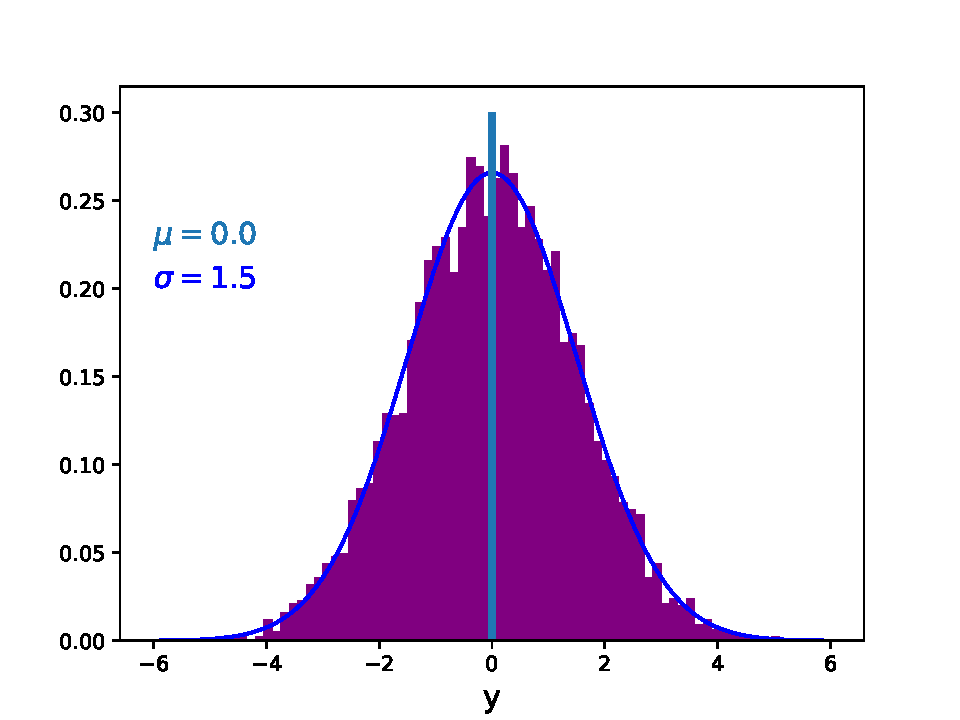
\includegraphics[scale=0.4]{gaussian_1d.pdf}
  \end{figure}
\end{frame}

\begin{frame}
  \frametitle{\secname}

  Loi Gaussienne multidimensionnelle (\coloredemph{vecteur} Gaussien): Distribution \coloredemph{jointe} des composantes d'un vecteur $d$-dimensionnel dont les \coloredemph{marginales} sont Gaussiennes (unidimensionnelles).
  \begin{equation*}
    \vectorx{Y} := [ y_1, \dots, y_d ]^\top  \sim \mathcal{N}(\vectorx{\mu} , \matrixx{\Sigma}) =  \frac{1}{\sqrt{(2 \pi)^d \det |\matrixx{\Sigma}|}} e^{-\frac{1}{2}(\vectorx{y - \mu})^\top \matrixx{\Sigma}^{-1} (\vectorx{y - \mu})}
  \end{equation*}
% 
  \begin{enumerate}
    \item $\vectorx{\mu} \in \mathbb{R}^d$: \coloredemph{vecteur moyen} $\implies \mu_j$: moyenne de la Gaussienne $y_j$
    \item $\matrixx{\Sigma} \in \mathbb{R}^{d \times d}$ définie positive\footnote{i.e. $\vectorx{a}^\top \matrixx{\Sigma} \vectorx{a} > 0$ (donc symmétrique)}: \coloredemph{matrice de covariance}
  \end{enumerate}
% 
  \pause
  \begin{equation*}
    \matrixx{\Sigma}
    =
    \begin{pmatrix} 
      \Sigma^2_{1}  & \Sigma_{{1}{2}} &  \cdots & \Sigma_{{1}{d}} \\
      \Sigma_{{2}{1}} & \ddots          & \cdots  & \vdots \\
      \vdots          & \vdots          & \ddots  & \vdots \\
      \Sigma_{{d}{1}} & \cdots          & \cdots  &  \Sigma^2_{d} 
      \end{pmatrix}
    \implies
    \left\{
      \begin{array}{ll}
        \Sigma_j  : \text{écart-type} \text{ de } y_j\\
        \Sigma_{ij} : \text{covariance entre les } \\
        \text{marginales de } y_i \text{ et } y_j
      \end{array}
    \right.
  \end{equation*}

  % $\mathcal{N}(\mu_1, \Sigma_1^2) \dots \mathcal{N}(\mu_d, \Sigma_d^2)$.
\end{frame}

% d=2, low correlation
\begin{frame}
  % \frametitle{\secname}
  Cas $d=2$:
  \begin{equation*}
    \vectorx{\mu}
    =
    \begin{pmatrix}
      \mu_1 \\
      \mu_2
    \end{pmatrix},
    \quad
    \matrixx{\Sigma}
    =
      \begin{pmatrix}
        \Sigma_{1} & \Sigma_{12} \\
        \Sigma_{21} & \Sigma_{2}
      \end{pmatrix}
    =
      \begin{pmatrix}
        1.5 & \color{red}\rho = -0.3 \\
        \color{red}\rho = -0.3 & 1.5
      \end{pmatrix}
  \end{equation*}
% 
  \begin{figure}
    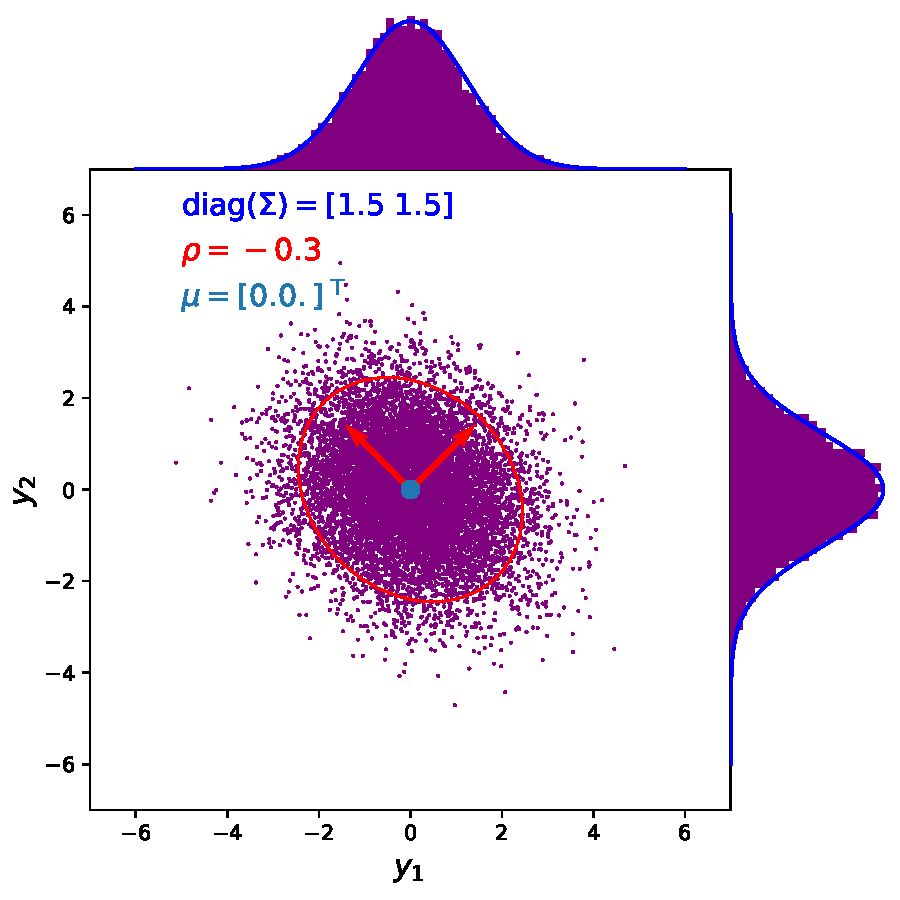
\includegraphics{gaussian_2d_rho_low.pdf}
  \end{figure}
\end{frame}

% d=2, high correlation
\begin{frame}
  Cas $d=2$:
  %
  \begin{equation*}
    \vectorx{\mu}
    =
    \begin{pmatrix}
      \mu_1 \\
      \mu_2
    \end{pmatrix},
    \quad
    \matrixx{\Sigma}
    =
      \begin{pmatrix}
        \Sigma_{1} & \Sigma_{12} \\
        \Sigma_{21} & \Sigma_{2}
      \end{pmatrix}
    =
      \begin{pmatrix}
        1.5 & \color{red}\rho = 1.1 \\
        \color{red}\rho = 1.1 & 1.5
      \end{pmatrix}
  \end{equation*}
% 
  \begin{figure}
    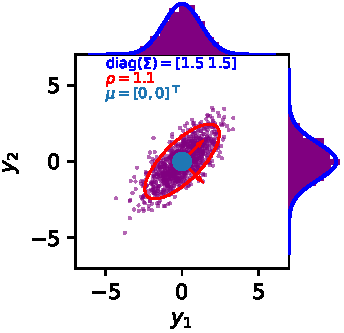
\includegraphics{gaussian_2d_rho_high.pdf}
  \end{figure}
\end{frame}

% d=2, zero correlation
\begin{frame}
  Cas $d=2$:
  %
  \begin{equation*}
    \vectorx{\mu}
    =
    \begin{pmatrix}
      \mu_1 \\
      \mu_2
    \end{pmatrix},
    \quad
    \matrixx{\Sigma}
    =
      \begin{pmatrix}
        \Sigma_{1} & \Sigma_{12} \\
        \Sigma_{21} & \Sigma_{2}
      \end{pmatrix}
    =
      \begin{pmatrix}
        1.5 & \color{red}\rho = 0 \\
        \color{red}\rho = 0 & 1.5
      \end{pmatrix}
  \end{equation*}
% 
  \begin{figure}
    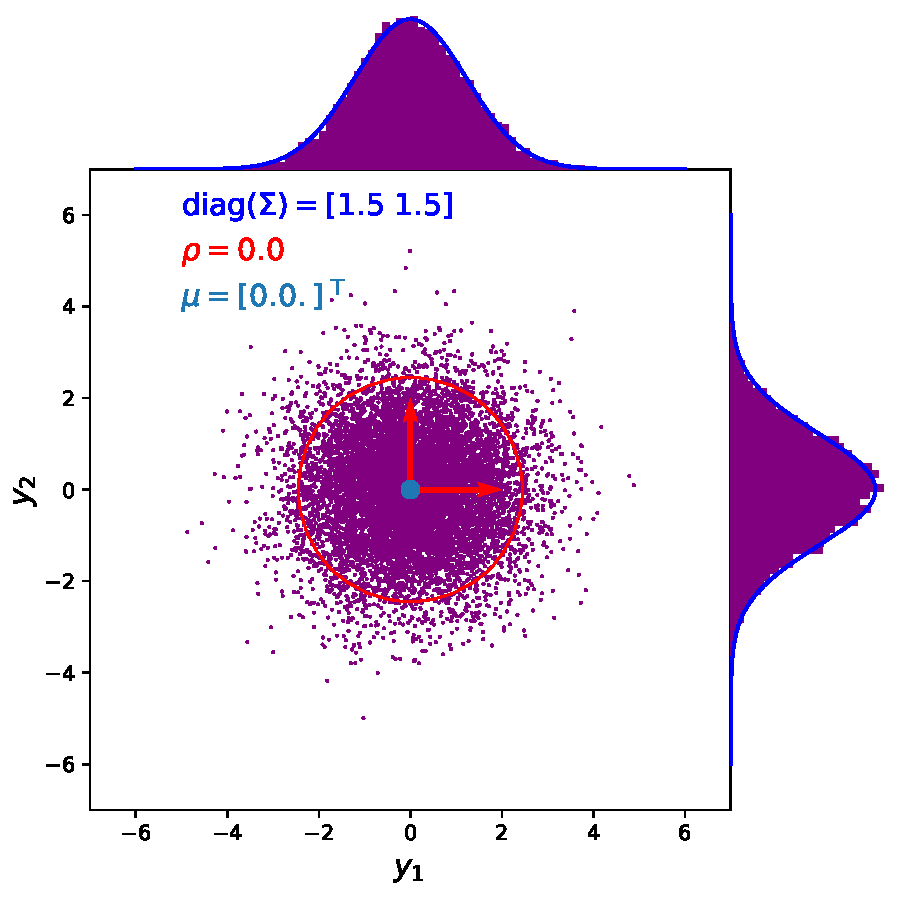
\includegraphics{gaussian_2d_rho_null.pdf}
  \end{figure}
\end{frame}

% d=5, high correlation: scatter and index plots
\begin{frame}
  % \frametitle{\secname}
  Cas $d=2$:
  %
  \begin{equation*}
    \vectorx{\mu}
    =
    \begin{pmatrix}
      0 \\
      0 \\
      \dots
    \end{pmatrix},
    \quad
    \matrixx{\Sigma}
    =
    \begin{pmatrix}
      1.5 & 0.99 & \color{lightgray}0.98 & \color{lightgray}0.96 & \color{lightgray}0.94 \\
      0.99 & 1.5 & \color{lightgray}0.99 & \color{lightgray}0.98 & \color{lightgray}0.96 \\
      \color{lightgray}0.98 & \color{lightgray}0.99 & \color{lightgray}1.5 & \color{lightgray}0.99 & \color{lightgray}0.98 \\
      \color{lightgray}0.96 & \color{lightgray}0.98 & \color{lightgray}0.99 & \color{lightgray}1.5 & \color{lightgray}0.99 \\
      \color{lightgray}0.94 & \color{lightgray}0.96 & \color{lightgray}0.98 & \color{lightgray}0.99 & \color{lightgray}1.5
      \end{pmatrix}
  \end{equation*}
  %
  \begin{figure}[ht]
    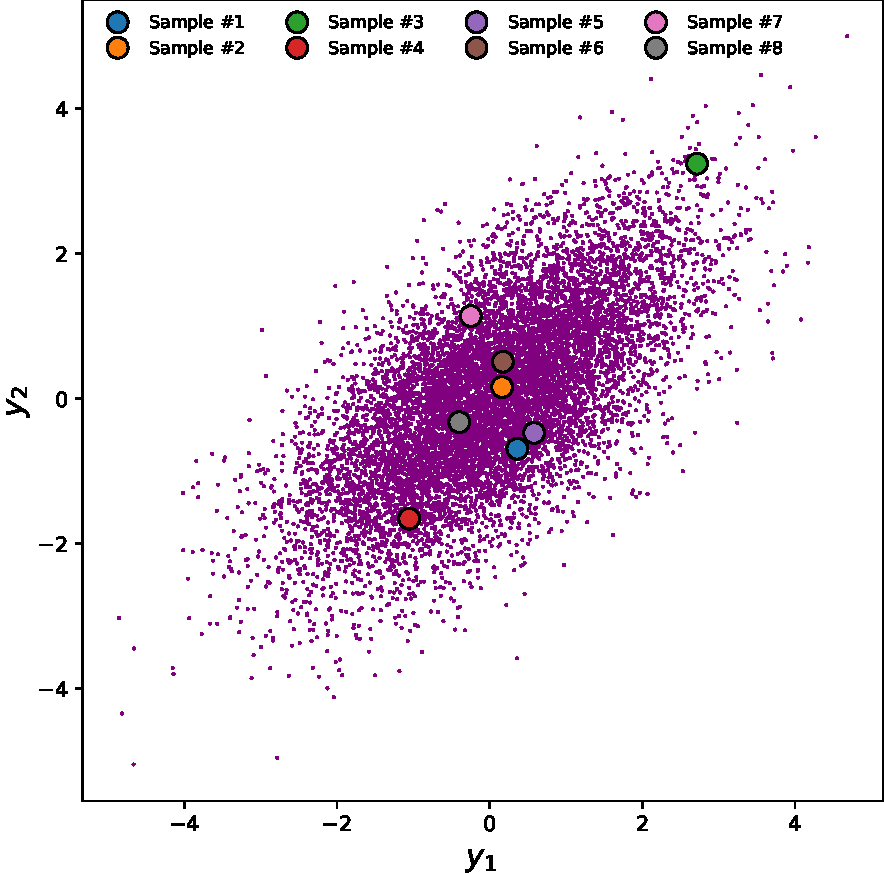
\includegraphics[scale=0.3]{gaussian_2d_2outof5.pdf}
    $\Longleftrightarrow$
    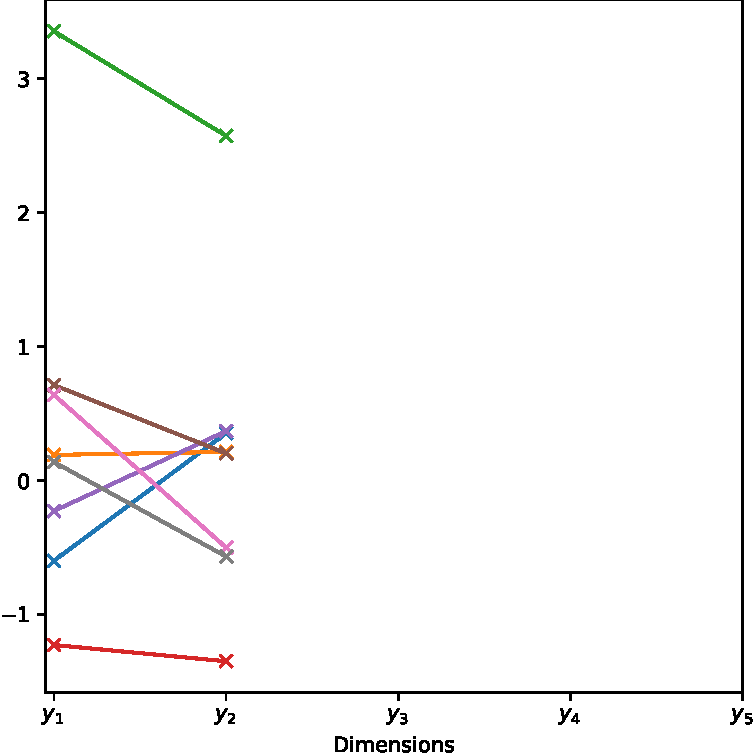
\includegraphics[scale=0.3]{gaussian_2d_valuevsindex.pdf}
    \caption{Dimensions $j=1, 2$. Gauche: \textcolor{violet}{$10^4$} $+8$ échantillons. 
    Droite: $8$ \coloredemph{mêmes} échantillons.}
  \end{figure}
\end{frame}

% d=5, high correlation: scatter and index plots
\begin{frame}
  Cas $d=5$:
  %
  \begin{equation*}
    \vectorx{\mu}
    =
    \begin{pmatrix}
      0 \\
      0 \\
      \dots
    \end{pmatrix},
    \quad
    \matrixx{\Sigma}
    =
    \begin{pmatrix}
      1.5 & 0.99 & 0.98 & 0.96 & 0.94 \\
      0.99 & 1.5 & 0.99 & 0.98 & 0.96 \\
      0.98 & 0.99 & 1.5 & 0.99 & 0.98 \\
      0.96 & 0.98 & 0.99 & 1.5 & 0.99 \\
      0.94 & 0.96 & 0.98 & 0.99 & 1.5
      \end{pmatrix}
  \end{equation*}
  %
  Chaque courbe est un tirage de $\mathcal{N}(\vectorx{\mu} , \matrixx{\Sigma})$
  \begin{figure}[ht]
    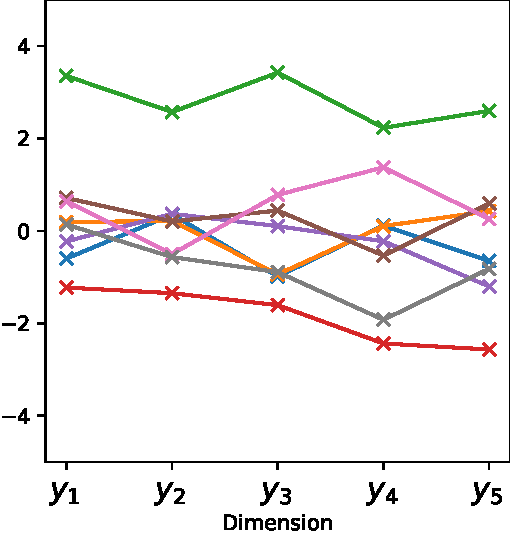
\includegraphics[scale=0.3]{gaussian_5d_valuevsindex.pdf}
    \caption{$8$ échantillons, dimensions $j=1, \dots, 5$}
  \end{figure}
\end{frame}

% d=50, high correlation: scatter and index plots
\begin{frame}
  Cas $d=50$:
  %
  \begin{equation*}
    \vectorx{\mu}
    =
    \begin{pmatrix}
      0 \\
      0 \\
      \dots
    \end{pmatrix},
    \quad
    \matrixx{\Sigma}
    =
    \scalemath{0.65}{
      \begin{pmatrix}
        1.5 & 0.998 & 0.993 & 0.986 & 0.975 & 0.962 & 0.946 & 0.927 & \cdots \\
        0.998 & 1.5 & 0.998 & 0.993 & 0.986 & 0.975 & 0.962 & 0.946 & \cdots \\
        0.993 & 0.998 & 1.5 & 0.998 & 0.993 & 0.986 & 0.975 & 0.962 & \cdots \\
        0.986 & 0.993 & 0.998 & 1.5 & 0.998 & 0.993 & 0.986 & 0.975 & \cdots \\
        0.975 & 0.986 & 0.993 & 0.998 & 1.5 & 0.998 & 0.993 & 0.986 & \cdots \\
        0.962 & 0.975 & 0.986 & 0.993 & 0.998 & 1.5 & 0.998 & 0.993 & \cdots \\
        0.946 & 0.962 & 0.975 & 0.986 & 0.993 & 0.998 & 1.5 & 0.998 & \cdots \\
        0.927 & 0.946 & 0.962 & 0.975 & 0.986 & 0.993 & 0.998 & 1.5   \\
        \hdots & \hdots & \hdots & \hdots & \hdots & \hdots & \hdots & \hdots & 1.5
      \end{pmatrix}
    }
  \end{equation*}
  Chaque courbe est un tirage de $\mathcal{N}(\vectorx{\mu} , \matrixx{\Sigma})$
  %
  \begin{figure}[ht]
    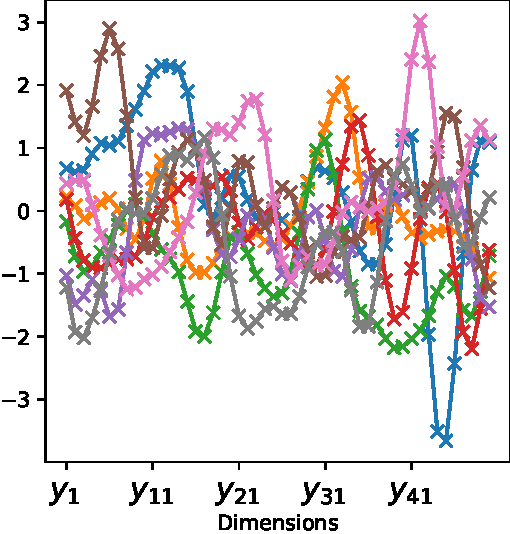
\includegraphics[scale=0.3]{gaussian_50d_valuevsindex.pdf}
    \caption{$8$ échantillons, dimensions $j=1, \dots, 50$}
  \end{figure}
\end{frame}
%

% GP definition
\begin{frame}
  \frametitle{\secname}
  Cas $d=\infty$: chaque courbe est une \coloredemph{collection infinie} de valeurs, que l'on peut voir comme une fonction:
  %
  \begin{enumerate}
    \item $\vectorx{\mu}$: vecteur de taille infinie $\Leftrightarrow$ fonction moyenne $\mathbb{E}(y(x)) = m(\vectorx{x})$
    \item $\matrixx{\Sigma}$: matrice de taille infinie $\Leftrightarrow$  noyau de covariance 
    $\mathbb{C}( y(\vectorx{x}), y(\vectorx{x^\prime}) ) = k(\vectorx{x}, \vectorx{x^{\prime}})$
  \end{enumerate}
  % 
  \pause
  % 
  \begin{block}{Processus Gaussien $y(\vectorx{x}) \sim GP(m, k)$}
    Un processus Gaussien (GP) est une distribution de probabilités sur un espace de \coloredemph{fonctions},
    $y(\vectorx{x}): \mathcal{X} \to \mathcal{Y}$, telle que toute collection finie
    $[ y(x_i), \dots, y(x_j), \dots y(x_k) ], \forall i,j,k$ forme un vecteur Gaussien. 
    % Les deux fonctions $m$ et $k$ définissent les paramètres du $GP$.
  \end{block}
  \pause
  Exemple, $y(t): \mathbb{R} \to \mathbb{R}$ (série temporelle), \coloredemph{n'importe qu'elle discrétisation} de $y$ doit
   former un vecteur Gaussien, en prenant par ex $2$ entrées de $y$:
  \begin{equation*}
    y(\vectorx{x}) \sim GP(m, k) \implies
    y([t_i, t_j]) \sim \mathcal{N} (
      % mu
      \begin{pmatrix}
        \mu_i \\
        \mu_j 
      \end{pmatrix},
      % sigma
      \begin{pmatrix}
        \Sigma_{i}^2 & \Sigma_{ij} \\
        \Sigma_{ij} & \Sigma_{j}^2
      \end{pmatrix}
      )
  \end{equation*}
  %
\end{frame}

% informal details
\begin{frame}
  \frametitle{\secname}
  \begin{itemize}
    \item On impose souvent une forme simple sur $\mathbb{E}(y(x)) = m(x)$ 
    comme: $\vectorx{\beta}^\top \vectorx{x}$, $\vectorx{0}$
    \pause
    \item $y: \mathcal{X} \to \mathcal{Y}$ est une \coloredemph{fonction}: il suffit de bien choisir $\mathcal{X}$ et $\mathcal{Y}$
    \begin{itemize}
      \item $\mathcal{X} = \mathbb{R}^{+}$ et $\mathcal{Y} = \mathbb{R}$ $\implies$
      $y$ = \coloredemph{série temporelle}
      \pause
      \item $\mathcal{X} = [a, b] \times [c, d]$ et  $\mathcal{Y} = \mathbb{R}$ $\implies$
      $y$ = \coloredemph{champ spatial} (météo, hydro, etc)
      \pause
      \item $\mathcal{X} = [a, b] \times [c, d] \times \mathbb{R}^{+}$ et $\mathcal{Y} = \mathbb{R}$ $\implies$
      $y$ = \coloredemph{série temporelle d'images}
      \pause
      \item $\mathcal{X} = \mathbb{R}^{d}$ et $\mathcal{Y} = \{1 \dots K \}$ $\implies$
      $y$ = \coloredemph{classificateur} d'images/pixels (ex: segmentation, catégorisation)
      \item $\mathcal{X}$ et $\mathcal{Y}$ peuvent être des espaces de graphes
      \item \dots etc, etc, etc.
    \end{itemize}
  \end{itemize}
  % 
\end{frame}

\subsection{Le kernel}
\begin{frame}
  \frametitle{\secname}
  % 
  \begin{itemize}
    \item $k(\vectorx{x}, \vectorx{x^{\prime}}) = \mathbb{C}( y(\vectorx{x}), y(\vectorx{x^\prime}) )$
     représente la \coloredemph{similarité de $y$} entre deux entrées $\vectorx{x}$ et $\vectorx{x}^\prime$,
     donc doit générer une matrice de covariance valide
     \footnote{
      $\sum_{i,j}^{n} a_i a_j k(\vectorx{x}_i, \vectorx{x}_j) \geq 0, \forall \vectorx{a} = [a_1, \dots, a_n]$
    }
    \pause
    \item $k$ défini \coloredemph{implicitement} les propriétés fonctionnelles de $y$
    \footnote{
      C-à-d être un noyau reproduisant d'un espace de Hilbert:
      $y(x_0) = \sum_{i=1}^{\infty} y(x_i) k(x_i, x_0)$ 
    }
    \pause
    \item Un kernel est dépend d'un vecteur \coloredemph{d'hyperparamètres} $\vectorx{\theta}$
    \pause
    \item Et donc le nerf d'un $GP$ est essentiellement dans son kernel (noyau)
  \end{itemize}
\end{frame}

% Examples of kernel functions
\begin{frame}
  \frametitle{\secname}
  \begin{itemize}
    \item Quelques exemples de $GP(0, k)$ défini sur $\mathcal{X} = \mathbb{R}^+$ et $\mathcal{Y} = \mathbb{R}$
    (série temporelle)
    \item kernel de série temporelle $\leftrightarrow$ fonction d'autocovariance
    \item Visualiser: bonne manière de comprendre un kernel (au delà des considérations théoriques...)
  \end{itemize}  
\end{frame}

% Exponential quadratic
\begin{frame}
  \frametitle{\secname}
  \begin{itemize}
    \item Exponentiel quadratique (aka "Radial basis", "Gaussian", "Heat" kernel):
    $k (t, t^\prime) = e^{- \frac{(t - t^\prime)^2}{2 \ell^2} }$
  \end{itemize}
  %
  \begin{figure}
    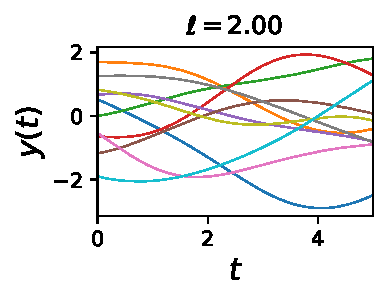
\includegraphics{10_gp_time_SquaredExponentialKernel_2.00.pdf}
  \end{figure}
\end{frame}

\begin{frame}
  \frametitle{\secname}
  % 
  \begin{itemize}
    \item Exponentiel quadratique (aka "Radial basis", "Gaussian", "Heat" kernel):
    $k (t, t^\prime) = e^{- \frac{(t - t^\prime)^2}{2 \ell^2} }$
  \end{itemize}
  %
  \begin{figure}
    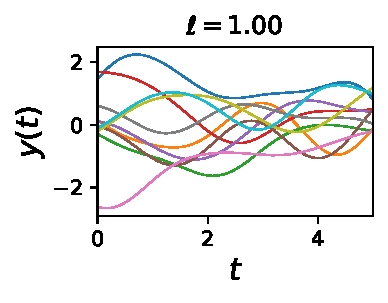
\includegraphics{10_gp_time_SquaredExponentialKernel_1.00.pdf}
  \end{figure}
\end{frame}

\begin{frame}
  \frametitle{\secname}
  % 
  \begin{itemize}
    \item Exponentiel quadratique (aka "Radial basis", "Gaussian", "Heat" kernel):
    $k (t, t^\prime) = e^{- \frac{(t - t^\prime)^2}{2 \ell^2} }$
    \item $GP (0, k)$ génères des $y$ infiniment différentiables par rapport à $t$
    \item \implies $\ell$ contrôle le lissé (ici au sens oscillatoir) des générées
  \end{itemize}
  %
  \begin{figure}
    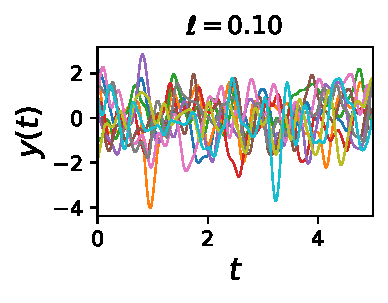
\includegraphics{10_gp_time_SquaredExponentialKernel_0.10.pdf}
  \end{figure}
\end{frame}

% Matern kernel
\begin{frame}
  \frametitle{\secname}
  % 
  \begin{itemize}
    \item kernel de Matérn:
    $k (t, t^\prime) = ( 1 + \sqrt{\frac{3 |t - t^\prime|}{\ell} } ) e^{-\sqrt{\frac{3 |t - t^\prime|}{\ell} }}$
  \end{itemize}
  %
  \begin{figure}
    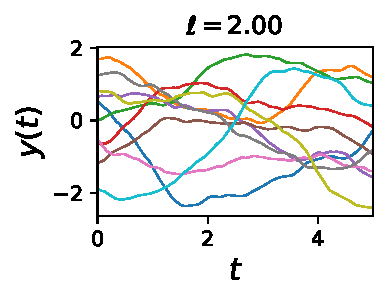
\includegraphics{10_gp_time_MaternKernel_2.00.pdf}
  \end{figure}
\end{frame}

\begin{frame}
  \frametitle{\secname}
  % 
  \begin{itemize}
    \item kernel de Matérn:
    $k (t, t^\prime) = ( 1 + \sqrt{\frac{3 |t - t^\prime|}{\ell} } ) e^{-\sqrt{\frac{3 |t - t^\prime|}{\ell} }}$
  \end{itemize}
  %
  \begin{figure}
    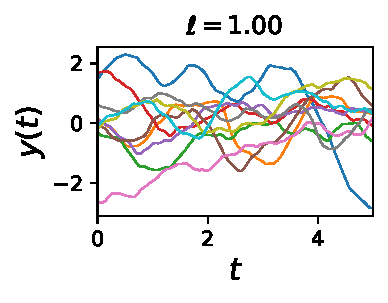
\includegraphics{10_gp_time_MaternKernel_1.00.pdf}
  \end{figure}
\end{frame}

\begin{frame}
  \frametitle{\secname}
  % 
  \begin{itemize}
    \item kernel de Matérn:
    $k (t, t^\prime) = ( 1 + \sqrt{\frac{3 |t - t^\prime|}{\ell} } ) e^{-\sqrt{\frac{3 |t - t^\prime|}{\ell} }}$
    \item Génère des $y$ différentiables une seule fois par rapport à $t$
    \item $\ell$: même interprétation que le kernel exponentiel quadratique
  \end{itemize}
  %
  \begin{figure}
    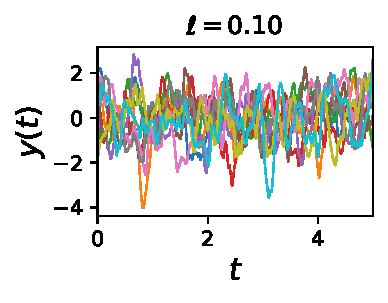
\includegraphics{10_gp_time_MaternKernel_0.10.pdf}
  \end{figure}
\end{frame}

% Locally periodic
\begin{frame}
  \frametitle{\secname}
  % 
  \begin{itemize}
    \item kernel locallement-périodique:
    $k (t, t^\prime) = e^{- \frac{2 \sin^2(\pi (t - t^\prime) / p)}{\ell^2}}$ %$e^{- \frac{(t - t^\prime)^2}{2 \ell^2}} $
  \end{itemize}
  %
  \begin{figure}
    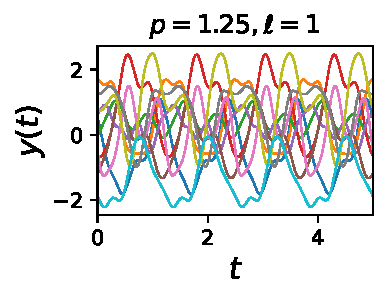
\includegraphics{10_gp_time_PeriodicKernel_1.25.pdf}
  \end{figure}
\end{frame}

\begin{frame}
  \frametitle{\secname}
  % 
  \begin{itemize}
    \item kernel locallement-périodique:
    $k (t, t^\prime) = e^{- \frac{2 \sin^2(\pi (t - t^\prime) / p)}{\ell^2}}$ %$e^{- \frac{(t - t^\prime)^2}{2 \ell^2}} $
    \item Génère des $y$ quasi-périodiques
  \end{itemize}
  %
  \begin{figure}
    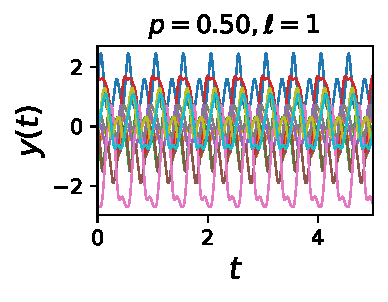
\includegraphics{10_gp_time_PeriodicKernel_0.50.pdf}
  \end{figure}
\end{frame}

% 
\begin{frame}
  \frametitle{\secname}
  %
  \begin{itemize}
    \item Aussi, des kernels dans le domaine fréquentiel (Fourier)
    \footnote{ex: $\sum_{q=0}^Q \sigma_q^2 e^{-2 \pi^2 \Sigma_q (t-t^\prime)^2} \cos(2\pi \mu_q (t-t^\prime))$}
  %  
  \pause
    \item Une famille standard est celle des \coloredemph{kernels stationnaires}. 
    $k(t, t^\prime)$ ne dépend que de $t - t^\prime$ (ex: tous les kernels précédents):
  \end{itemize}
  %
  \begin{figure}
    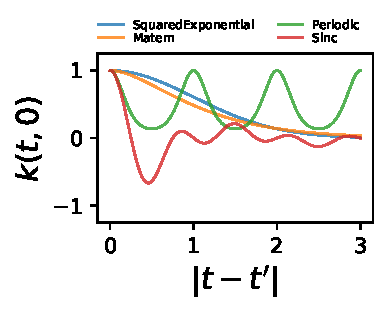
\includegraphics[scale=0.80]{autocov_gp_1D.pdf}
  \end{figure}
\end{frame}

\begin{frame}
  \frametitle{\secname}
  %
  \begin{itemize}
    \item Fléxibilité des kernels: $k_1 + k_2$, $k_1 \times k_2$, $g(t) \times k$ ($g$ est déterministe)
  %
  \pause
    \item Depuis quelques années: construction de kernels par des deep-nets (deep-kernel)
  % 
  \pause
    \item Plus récemment: construction du kernel à  partir d'équations différentielles
  \end{itemize}
\end{frame}

%========== Fitting a GP ==================%
\section{Utilisation}

% Gaussian Bayesian rule
\subsection{Règle de Bayes}
\begin{frame}
  \frametitle{\secname}
\begin{itemize}
  \item<1-> Règle de Bayes: 
  $p(y_2| y_1)
  = \frac{p(y_1, y_2)}{p(y_1)}
  = \frac{p(y_1 | y_2) p(y_2)}{p(y_1)}
  $%
  \item<2-> $  \vectorx{y} = [y_1, y_2]^\top \sim \mathcal{N} (
    \begin{pmatrix}
      \mu_1 \\
      \mu_2
    \end{pmatrix},
      \begin{pmatrix}
        \Sigma_{1} & \Sigma_{12} \\
        \Sigma_{12} & \Sigma_{2}
      \end{pmatrix}
  )$%
  \item<3-> $
  p(y_2 | y_1 = u) = \mathcal{N} (
    \mu_2 \coloredemph{+ \Sigma_{12} \Sigma_1^{-1} (u - \mu_1)}
    ,
    \Sigma_2 \coloredemph{- \Sigma_{12}^2 \Sigma_1^{-1}}
  )$%
\end{itemize}
\begin{figure}
\only<4>{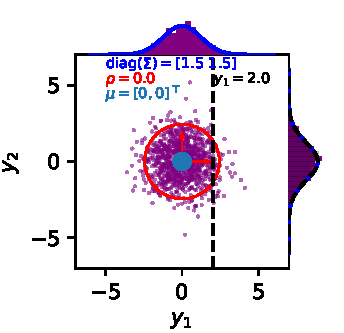
\includegraphics{gaussian_2d_rho_null_with_conditional.pdf}}%
\only<5>{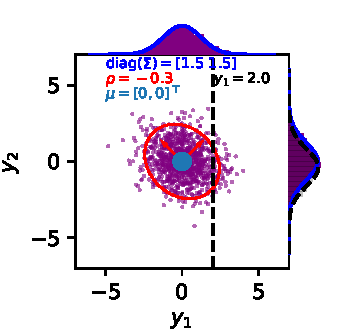
\includegraphics{gaussian_2d_rho_low_with_conditional.pdf}}%
\only<6>{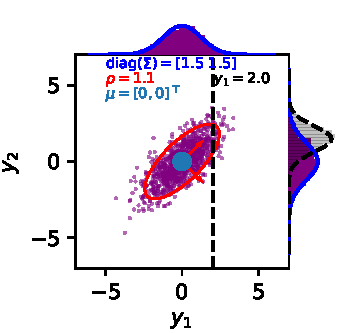
\includegraphics{gaussian_2d_rho_high_with_conditional.pdf}}%
\end{figure}
\end{frame}
%
\subsection{prédiction = data $\times$ hypothèse}
\begin{frame}
  \begin{itemize}
    \item<1-> Data: $\{y_i, x_i\}_{1 \leq i \leq n}$
    \item<2-> Modèle de prédiction: $\tilde{y}(x_0) = f(x_0) + \epsilon$
    % \item Modèle des données d'entraînement: $y_i = f(x_i) + \epsilon$
    % \pause
    \item<3-> Hypothèse: $f$ est un processus Gaussien
    \item<4-> $prédiction = hypothèse + data + bruit$
    \item<5-> But: aprendre $f$ et prédire $\tilde{y}(x_0)$
    \item<6-> Règle de Bayes:
      \begin{equation*}
        \begin{split}
        % informal way
        \only<7>{
          p(hypothèse | data)
          & = \frac{
            p(data, hypothèse)
          }{
            p(data)
          } \\
          & =
          \frac{
            \overbrace{p(data | hypothèse)}^{\textcolor{red}{likelihood}}
            \overbrace{p(hypothèse)}^{\textcolor{red}{a priori}}
          }{
            p(data)
          }
        }
        % formal way
        \only<8>{
          p(f | X, y)
        & =
        }
        \end{split}
      \end{equation*}
  \end{itemize}
\end{frame}

\subsection{GP: fondamentalement Bayésien}
% Color: current +/- prior with underbrace
\begin{frame}
  \frametitle{\secname}
\begin{itemize}
  \item Règle de Bayes étendue aux $GP$: $y \sim GP(m_y, k_y)$ et $f \sim GP(0, k_f)$
  \pause
    \begin{equation*}
      y | f(x_1) \dots f(x_n) \sim GP(m^*, k^*) \\
    \pause
      \matrixx{K}_{fn}
      =
      \scalemath{0.80}{
        \coloredemph{
      \begin{pmatrix}
        k_f(x_1, x_1) & \dots & k_f(x_1, x_n) \\
        \vdots      & \ddots& \vdots          \\
        k_f(x_n, x_1) & \dots & k_f(x_n, x_n)
      \end{pmatrix}}}\\
      \pause
      % posterior mean
      m^* (u) = m_y (u) + 
      \pause
      \scalemath{0.80}{
      \coloredemph{
        [k_y(u, x_1), \dots, k_y(u, x_n)]
      \matrixx{K}_{fn}^{-1}
      }%
      [f(x_1), \dots, f(x_n)]^\top%
      }\\
      \pause
      % posterior covariance
      k^* (u, u^\prime) = k_y (u, u^\prime) -
      \pause
      \scalemath{0.80}{
      \coloredemph{
        [k_y(u, x_1), \dots, k_y(u, x_n)]
      \matrixx{K}_{fn}^{-1}
      }
      [k_y(u^\prime, x_1), \dots, k_y(u^\prime, x_n)]^\top
      }%
    \end{equation*}
\end{itemize}
\end{frame}

%========== Motivations ==================%
\section{Motivations}
\subsection{Tractabilité mathématique}

% Mathematical properties
\begin{frame}
  \frametitle{\secname}
$y_1 \sim GP$, $y_2 \sim GP$
\begin{itemize}
  \pause
  \item Somme: $y_1 + y_2 \sim GP$
  %
  \pause
  \item Opérateur linéaire $\mathcal{L}$ (gradient, $\int$, eq-diff linéaire, etc.):
  $\mathcal{L}y_1 \sim GP$
  % 
  \item Bayésien $\implies$ probabiliste: accès à l'incertitude de prédiction
  \pause
  \item Conditionnement Bayésien: $y_1 | y_2 \sim GP$ (\coloredemph{important}, détails plus tard)
  % 
  \pause
  \item Connaissant uniquement moyenne et covariance de $\vectorx{u}$ et $\vectorx{v}$,
  on montre que la meilleure prédiction (en moyenne) est Gaussienne (maximum d'entropie).
\end{itemize}
\end{frame}

% Non-parametric
\subsection{Non-paramétrique}
\begin{frame}
  \frametitle{\secname}
    \begin{itemize}
    \item Modèle \coloredemph{paramétrique}: modèle = des paramètres
    \item Les données d'entraînement \coloredemph{conditionnent} les paramètres qui conditionnent eux-mêmes l'inférence (lien indirect)
    \pause
    \item Ex: régression linéaire, réseau de neurones (poids), K-means, RF
    \pause
    \item Modèle \coloredemph{non-paramétrique}: modèle = des données
    \item Les données d'entraînement \coloredemph{conditionnent} l'inférence (lien direct)
    \pause
    \item Ex: SVM, k-NN, \coloredemph{GP} ($\coloredemph{\matrixx{K}_{fn}^{-1}}$)
    \pause
    %
    \item Avantages du non-paramétrique:
      \begin{enumerate}
        \item apprentissage "direct" de la distribution des observations
        \item théorie: $n \to \infty$: le modèle se trompe de moins en moins (pas toujours le cas du paramétrique)
        \item inférence Gaussienne optimale\footnote{à partir de moyenne et covariance uniquement.}
      \end{enumerate}
    \pause
    %
    Inconvénivents du non-paramétrique:
      \begin{enumerate}
        \item risque d'overfit plus important
        \item variance de prédiction sensible aux hyperparamètres du kernel
        \item inférence plus coûteuse en général
      \end{enumerate}
  \end{itemize}
\end{frame}

%========== Application ==================%
\section{Application}

\secction{GP pour les données non-Gaussiennes}
\end{document}